\begin{figure}[t]
	\centering
	\begin{subfigure}{0.31\textwidth}
		\centering
		\includegraphics[width=\textwidth]{figures/K1-posterior-W.pdf}
		% \caption{K1 ($F$: 0.9102)}
		\caption{K1}
	\end{subfigure}
	\begin{subfigure}{0.31\textwidth}
		\centering
		\includegraphics[width=\textwidth]{figures/K3-posterior-W.pdf}
		% \caption{K3 ($F$: 0.7763)}
		\caption{K3}
	\end{subfigure}
	\begin{subfigure}{0.31\textwidth}
		\centering
		\includegraphics[width=\textwidth]{figures/K4-posterior-W.pdf}
		% \caption{K4 ($F$: 0.8315)} 
		\caption{K4} 
	\end{subfigure}
	\begin{subfigure}{0.31\textwidth}
		\centering
		\includegraphics[width=\textwidth]{figures/K5-posterior-W.pdf}
		% \caption{K5 ($F$: 0.7799)}
		\caption{K5}
	\end{subfigure}
	\begin{subfigure}{0.31\textwidth}
		\centering
		\includegraphics[width=\textwidth]{figures/K9-posterior-W.pdf}
		% \caption{K9 ($F$: 0.7219)}
		\caption{K9}
	\end{subfigure}
	\begin{subfigure}{0.31\textwidth}
		\centering
		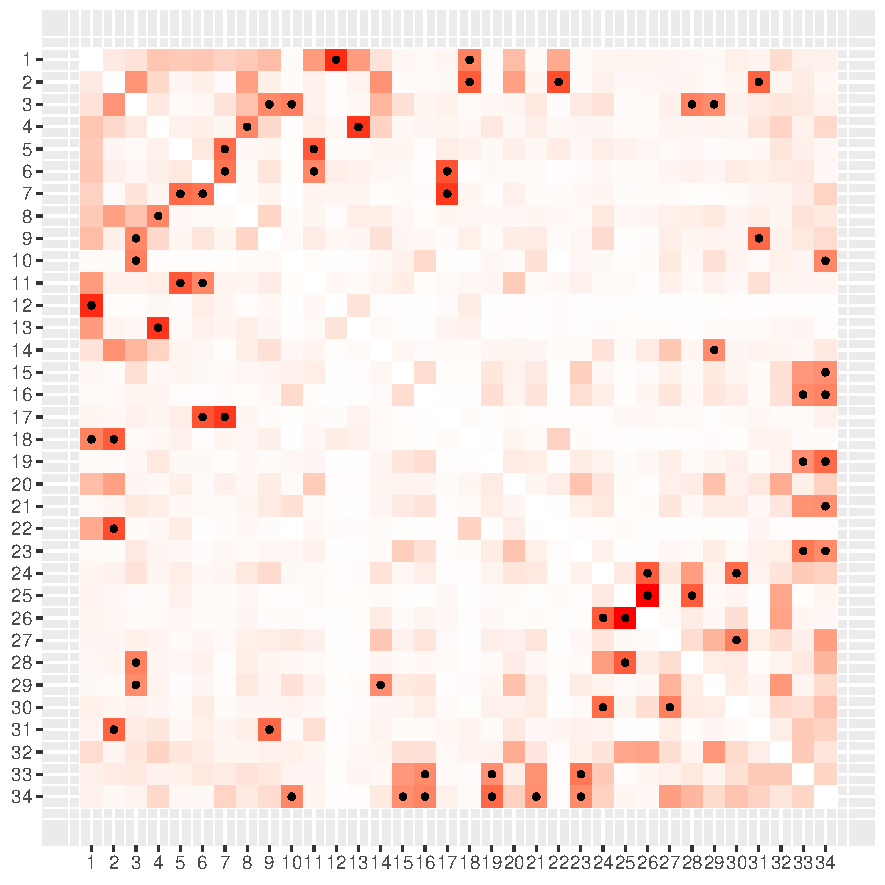
\includegraphics[width=\textwidth]{figures/K10-posterior-W.pdf}
		% \caption{K10 ($F$: 0.7838)}
		\caption{K10}
	\end{subfigure}
	\caption{Posterior Adjacency Matrices.}
	\label{fig:K-posterior-1}
\end{figure}
